\begin{figure}[H]
	\centering
	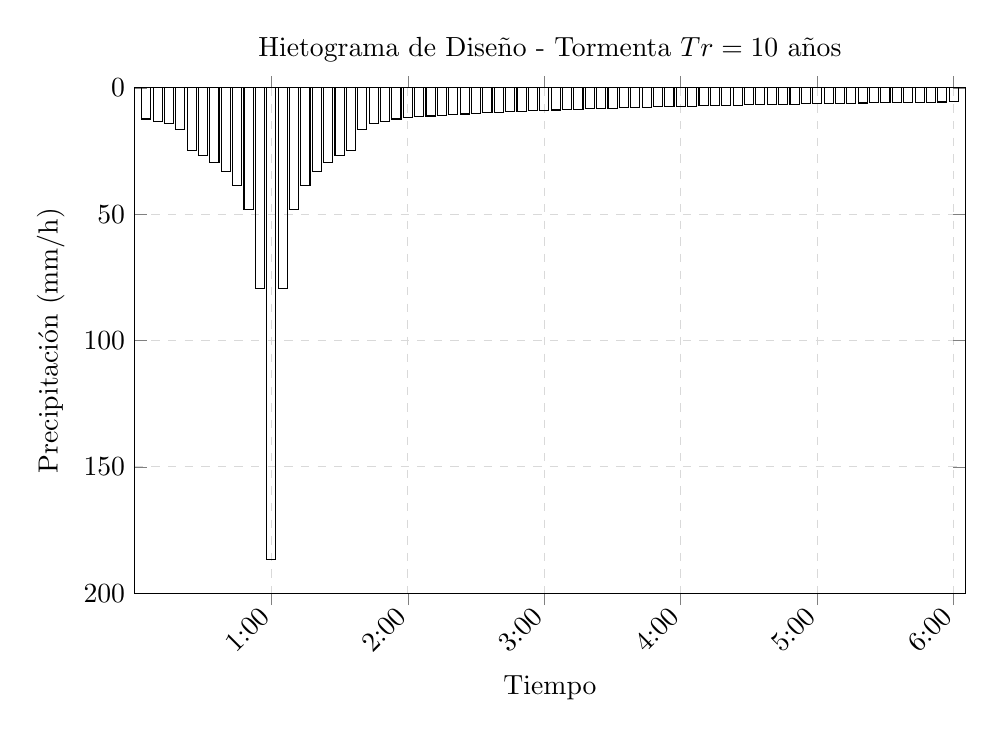
\begin{tikzpicture}
		\begin{axis}[
			title={Hietograma de Diseño - Tormenta $\text{Tr}=10$ años},
			width=\textwidth,
			height=8cm,
			xlabel={Tiempo},
			ylabel={Precipitación (mm/h)},
			y dir=reverse,
			ymin=0,
			ymax=200,
			xmin=0,
			xmax=365,
			ybar,
			bar width=4,
			xtick={60, 120, 180, 240, 300, 360},
			xticklabels={1:00, 2:00, 3:00, 4:00, 5:00, 6:00},
			xticklabel style={rotate=45, anchor=east},
			grid=major,
			grid style={dashed, gray!30},
			]
			\addplot [
			draw=black,
			fill=none
			]
			coordinates {
				(5, 12.33) (10, 13.16) (15, 14.13) (20, 16.43) (25, 24.81) (30, 26.88)
				(35, 29.57) (40, 33.23) (45, 38.66) (50, 47.96) (55, 79.26) (60, 186.64)
				(65, 79.26) (70, 47.96) (75, 38.66) (80, 33.23) (85, 29.57) (90, 26.88)
				(95, 24.81) (100, 16.43) (105, 14.13) (110, 13.16) (115, 12.33) (120, 11.79)
				(125, 11.46) (130, 11.15) (135, 10.86) (140, 10.59) (145, 10.34) (150, 10.10)
				(155, 9.87) (160, 9.66) (165, 9.45) (170, 9.26) (175, 9.08) (180, 8.90)
				(185, 8.74) (190, 8.58) (195, 8.42) (200, 8.28) (205, 8.14) (210, 8.01)
				(215, 7.88) (220, 7.75) (225, 7.63) (230, 7.52) (235, 7.41) (240, 7.30)
				(245, 7.20) (250, 7.10) (255, 7.00) (260, 6.91) (265, 6.82) (270, 6.74)
				(275, 6.65) (280, 6.57) (285, 6.49) (290, 6.41) (295, 6.34) (300, 6.27)
				(305, 6.19) (310, 6.13) (315, 6.06) (320, 5.99) (325, 5.93) (330, 5.87)
				(335, 5.81) (340, 5.75) (345, 5.69) (350, 5.64) (355, 5.58) (360, 5.53)
			};
		\end{axis}
	\end{tikzpicture}
	\caption{Hietograma de la lluvia de diseño para un período de retorno de 10 años.}
	\label{fig:hietograma_tr10}
\end{figure}

